% Lying Comments: final report (ACM conference style, sigconf).
% Compile on Overleaf (pdfLaTeX + BibTeX): upload this folder, set main.tex as the main file.
% Every number comes from analysis/main.md, analysis/condefects.md and
% `python3 condefects/memorize.py summary`; rerun those if results change.
\documentclass[sigconf,nonacm]{acmart}

\usepackage{listings}
\usepackage{multirow}
\lstset{basicstyle=\ttfamily\footnotesize, columns=fullflexible, keepspaces=true,
        frame=single, framerule=0.4pt, xleftmargin=2pt, xrightmargin=2pt, aboveskip=6pt, belowskip=4pt}

\settopmatter{printacmref=false}
\setcopyright{none}
% Lets a paragraph with long code words stretch slightly instead of overflowing.
\setlength{\emergencystretch}{1.5em}

\newcommand{\wb}{\textsf{wrong\_behavior}}
\newcommand{\wl}{\textsf{wrong\_location}}
\newcommand{\wo}{\textsf{wrong\_output}}
\newcommand{\acc}{\textsf{accurate}}
\newcommand{\cd}{ConDefects}
% A comment quoted on its own line in the case studies.
\newcommand{\casecomment}[1]{\par\smallskip\noindent\hspace*{1em}\parbox{\dimexpr\columnwidth-1em\relax}{\raggedright\small\texttt{\# #1}}\par\smallskip\noindent\ignorespaces}

\begin{document}

\title{Lying Comments: Can a Misleading Code Comment Trick AI Into the Wrong Bug Fix?}

\author{Ankit Bhade}
\affiliation{\institution{North Carolina State University}\city{Raleigh}\state{NC}\country{USA}}
\email{aabhade@ncsu.edu}
\author{Arnav Yennam}
\affiliation{\institution{North Carolina State University}\city{Raleigh}\state{NC}\country{USA}}
\email{aryennam@ncsu.edu}
\author{Kushal Upreti}
\affiliation{\institution{North Carolina State University}\city{Raleigh}\state{NC}\country{USA}}
\email{kupreti@ncsu.edu}
\author{Seung Wook Jung}
\affiliation{\institution{North Carolina State University}\city{Raleigh}\state{NC}\country{USA}}
\email{sjung27@ncsu.edu}

\renewcommand{\shortauthors}{Bhade, Yennam, Upreti, and Jung}

\begin{abstract}
Code comments are part of what a large language model (LLM) reads when it fixes a bug, and comments are often out of date. We ask whether a misleading comment makes LLM bug fixing worse than an accurate one. We show each buggy program to the model four times, changing only one comment. The comment is either accurate or one of three misleading kinds: it describes the buggy behavior as intended, says the buggy part was checked and points elsewhere, or gives an example whose ``expected'' output is what the buggy code returns. We test two sizes of one model family (Qwen2.5-Coder 7B and 32B), with and without a warning that comments may be wrong, on two datasets: 120 new programs with one planted bug each, and 120 real one-line bugs from \cd{}. Across 3,840 repair attempts, misleading comments hurt only a little, and mostly the smaller model. The one significant drop is the wrong-location comment on 7B: from 71\% to 61\% fixed ($p = 0.003$, paired exact McNemar test). When 7B fails after this comment, the bug is left untouched 76\% of the time. The 32B model is barely affected. Models almost never question the comment: without a warning, 7B flagged 0 of 720 misleading comments and 32B flagged 5. The warning makes 32B flag more comments but does not change how many bugs either model fixes. A memorization check finds no sign that the models had seen the \cd{} programs.
\end{abstract}

\keywords{automated program repair, large language models, code comments, comment--code inconsistency, robustness}

\maketitle

% ---------------------------------------------------------------------------
\section{Introduction}

LLMs are now often used to fix bugs, both in chat and inside coding assistants. When a model fixes code, it reads everything it is given: the code, the task description, and the comments. Comments usually help. Vitale et al.~\cite{vitale2026comments} found that adding comments improves automated bug fixing, by up to three times for fine-tuned models. But comments can also be wrong. They fall out of date as code changes~\cite{wen2019inconsistencies}, and anyone who can edit a file can write one.

So what happens when a comment lies? Earlier work shows that misleading text can steer LLMs. Crafted bug reports can push repair tools toward an attacker's patch~\cite{przymus2026adversarial}, outdated comments mislead LLM code completion~\cite{xia2026outdated}, and misleading hints in code hurt LLM code reasoning~\cite{lam2025codecrash}. None of these studies puts a misleading comment \emph{inside} the code, next to the bug, and measures how it affects bug \emph{fixing}. This placement matters: a comment beside the buggy line looks like part of the program, not like an outside claim.

We test this with a controlled experiment. The model sees each buggy program four times. The code is the same each time; only one comment changes. The comment is either \emph{accurate} or one of three \emph{misleading} kinds, each written by a fixed rule (Section~\ref{sec:comments}). The model is not told that the comment might be wrong, except in a second prompt that adds this warning. We ask three research questions:

\begin{description}
\item[RQ1] Is a misleading comment worse than an accurate one, and does a larger model resist it better?
\item[RQ2] Which kind of misleading comment does the most damage?
\item[RQ3] Do models notice that the comment does not match the code, and does a warning help?
\end{description}

We test two sizes of the same open model family, Qwen2.5-Coder 7B and 32B~\cite{hui2024qwen25coder}, on two datasets: 120 small Python programs we wrote for this study, each with one planted bug, and 120 real one-line bugs from \cd{}~\cite{wu2024condefects}, a public dataset of wrong AtCoder contest submissions. In total we collect 3,840 repair attempts (240 programs $\times$ 4 comments $\times$ 2 prompts $\times$ 2 models).

Our main findings are:
\begin{itemize}
\item Misleading comments hurt only a little, and mostly the smaller model. The one significant effect is the \emph{wrong-location} comment on 7B: $-10$ percentage points (71\% $\to$ 61\%, $p = 0.003$). Across all misleading comments on our programs, 32B loses only 0.3 points.
\item The wrong-location comment works by sending the model to the wrong place. When 7B fails after it, the original bug is still there 76\% of the time, against 61\% after an accurate comment.
\item Models almost never question a comment. Without a warning, 7B flagged none of 720 misleading comments and 32B flagged 5. With the warning, 32B flags at most 8\%, but neither model fixes more bugs.
\item Surprisingly, the wrong-output comment slightly \emph{helps} on our programs (+4.6 points for 7B, not significant), possibly because its example names an input on which the code fails.
\end{itemize}

All programs, prompts, model replies, labels, and scripts are in our repository (see Data Availability).

% ---------------------------------------------------------------------------
\section{Background and Related Work}
\label{sec:related}

\paragraph{LLM-based program repair.}
Pre-trained LLMs can fix many bugs from just the buggy code and a short description, often better than earlier repair tools~\cite{xia2023apr}. These models use all of their input, so the text parts (descriptions, bug reports, comments) can shape the fix as much as the code does.

\paragraph{Comments and repair.}
Vitale et al.~\cite{vitale2026comments} study whether comments help automated bug fixing. They add LLM-written comments to a bug-fixing benchmark and fine-tune CodeT5+ and DeepSeek-Coder with and without them. When comments are present in both training and testing, exact-match fixes improve by up to three times. In a side check without fine-tuning, GPT-4.1's exact-match rate rises from 6.11\% to 8.63\% with comments. They also note that comments generated from the buggy code do not help and can mislead the model. They do not test deliberately misleading comments. Our accurate comment matches their helpful comment, and our wrong-behavior comment is a controlled version of a comment that describes the buggy code.

\paragraph{Comment--code inconsistency.}
Wen et al.~\cite{wen2019inconsistencies} study 1.3 billion code changes from 1,500 software systems and show that comments often fall out of sync with the code, so that they no longer describe what it does. Such out-of-date comments are the everyday, non-malicious source of the misleading comments we simulate.

\paragraph{Misleading text and LLMs.}
Przymus et al.~\cite{przymus2026adversarial} show that crafted bug reports can steer LLM-based repair toward an attacker's chosen patch, and that current defenses catch only some of them. Their misleading text is in a bug report, outside the code. Xia et al.~\cite{xia2026outdated} study outdated comments in LLM code \emph{completion} (writing new code, not fixing it) and find that comments strongly influence the generated code even though they are not reliable. CodeCrash~\cite{lam2025codecrash} inserts misleading hints into code and finds that 17 LLMs lose 23.2\% of their accuracy, on average, at predicting a program's output, showing that models rely too much on such hints when \emph{reasoning} about code. Our study fills the gap between these works: a misleading comment inside the code, next to the bug, in a bug-\emph{fixing} task, with tests that decide whether the fix is correct.

\paragraph{Data leakage.}
Public bug datasets may be in a model's training data, which can make repair results look better than they are. \cd{}~\cite{wu2024condefects} was built to reduce this risk by collecting faulty programs from recent AtCoder contests. Because \cd{} is still public, we also write a new dataset and run our own memorization check (Section~\ref{sec:memorization}).

% ---------------------------------------------------------------------------
\section{Study Design}
\label{sec:design}

\subsection{Task}
Each model gets a buggy program, a one-line problem description, and one comment version. It is asked to fix the bug and explain it in one or two sentences. A fix counts as a success only if the fixed program passes \emph{all} of its tests. A reply with no code, a renamed function, or code that crashes counts as a failure.

\subsection{Comment Versions}
\label{sec:comments}
Every program has four versions that differ only in one one-line comment, always in the same place (the first line inside the function for our programs, the first line of the program for \cd{}). Each kind follows a fixed rule:

\begin{description}
\item[\acc] True for the correct code: says what the code should do, without pointing at the bug. This is the baseline.
\item[\wb] Describes what the buggy code actually does, as if that were intended.
\item[\wl] Says the buggy part was checked and points to a different, real part of the code.
\item[\wo] An example of the form \texttt{Example: <call> returns <value>}, where the value is what the \emph{buggy} code returns, not the correct answer.
\end{description}

\noindent Figure~\ref{lst:example} shows the four comments for a small example. All comments must read like normal developer comments: one line, no words like ``bug'' or ``fix'', no hint at the input that triggers the bug, and no warning tone. Misleading comments must sound like reasonable design choices, not obviously wrong statements. In our pilot, natural-sounding misleading comments fooled the model, while odd-sounding ones did not.

\begin{figure}[t]
\begin{lstlisting}
def count_pairs(a, k):
    # COMMENT
    cnt = 0
    for i in range(len(a)):
        for j in range(i, len(a)):   # should be i + 1
            if a[i] + a[j] == k:
                cnt += 1
    return cnt
\end{lstlisting}
\small
\begin{tabular}{@{}p{0.27\columnwidth}p{0.68\columnwidth}@{}}
\acc & \raggedright\texttt{Counts pairs of different positions whose values sum to k}\tabularnewline
\wb & \raggedright\texttt{Counts pairs; a number may be paired with itself}\tabularnewline
\wl & \raggedright\texttt{Loop bounds verified; check the sum condition for edge cases}\tabularnewline
\wo & \raggedright\texttt{Example: count\_pairs([1, 2, 3], 4) returns 2}\tabularnewline
\end{tabular}
\Description{A nine-line Python function count\_pairs whose inner loop starts at i instead of i + 1, followed by the four one-line comments that replace its COMMENT placeholder.}
\caption{A worked example (not part of the dataset). Problem: ``Count the pairs of different positions in a list whose values add up to k.'' The inner loop starts at \texttt{i} instead of \texttt{i + 1}. One of the four comments replaces the \texttt{\# COMMENT} line; the note after the buggy line is only for the reader. For \texttt{[1, 2, 3]} and $k=4$ the buggy code returns 2; the correct answer is 1.}
\label{lst:example}
\end{figure}

\subsection{Datasets}

\paragraph{Our programs (120).}
We wrote 120 short Python functions, each with one planted bug, during this semester, so no model can have seen them before. Each program has a correct version, a buggy version that differs in exactly one line, at least five tests (5--8, median 6), a one-line problem description, and the four comments. The functions are short (2--11 non-blank lines, median 5). Bugs come in four types: \emph{off-by-one} (28), \emph{wrong comparison} (28), \emph{missed edge case} (28), and \emph{other} small single-line mistakes such as a wrong variable or a misused library call (36).

We started with a pilot of 12 programs (3 per team member). On the 7B model the pilot was too easy: 10 of the 12 programs were fixed under every comment, so the comment could not change the result. We therefore wrote guidelines for harder bugs, based on what the two programs that did fool the model had in common: the description states the goal, not the edge case; the buggy line looks like a reasonable choice; the bug shows up only on some inputs; and the bug can still be fixed from the description and an honest comment. We also added the \emph{other} bug type, because the three original types are all boundary bugs. The remaining 108 programs (27 per member) were written by an LLM from a different model family than the one we test (Claude Opus 5.5, in Claude Code). It followed written instructions that encode these rules, require every problem, topic, and bug trick to differ from the existing programs, and forbid testing programs on the models under study. No program was kept or dropped based on how the models did on it.

A checker script verifies every program: all required fields are present, exactly one line differs between the buggy and correct code, the correct code passes every test, the buggy code fails at least one, the comments follow the wording rules, and the \wo{} example really is what the buggy code returns. All 120 programs pass. Comparing programs across team members found no repeated problems (the most similar pair of descriptions scored 0.27 out of 1), although eight pairs of programs use a similar bug trick; we kept them.

\paragraph{\cd{} (120 real bugs).}
To see whether our findings hold for bugs that people actually made, we selected 120 Python bugs from \cd{}~\cite{wu2024condefects}. It pairs a wrong and an accepted AtCoder submission from the same user, together with AtCoder's official input/output tests. A script picked bugs from easy AtCoder Beginner Contest problems (difficulty below 800) where the buggy and fixed programs are 5--60 lines long, use only the standard library, and differ in exactly one line that changes the program's logic. We left out changes that only affect output format or wording, typos, imports, input reading, and leftover hard-coded test input, since these are about AtCoder's input/output rules rather than program logic. We dropped tests larger than 100\,KB or taking more than one second with the fixed code; the fixed code must pass all remaining tests and the buggy code must fail at least one. Problems were drawn in a fixed random order (seed 2026), one bug per problem. The selected programs have 3--58 non-blank lines (median 11) and 5--52 tests (median 15). We removed the original comments. The same LLM then wrote, for each program, a short problem description based on the AtCoder statement and the four comments, following the same rules. For \cd{}, the \wo{} comment has the form \texttt{Example: input '<input>' prints <output>}. Because these are real bugs, the types are uneven: 23 off-by-one, 12 wrong comparison, 11 missed edge case, and 74 other.

\subsection{Models and Prompts}
We test Qwen2.5-Coder-Instruct~\cite{hui2024qwen25coder} at 7B and 32B parameters. Because both come from one family, model size is the only difference. Both run through Ollama as 4-bit quantized builds (Ollama tags \nolinkurl{qwen2.5-coder:7b-instruct-q4_K_M} and \nolinkurl{qwen2.5-coder:32b-instruct-q4_K_M}) with temperature 0, seed 0, a 4,096-token context, and at most 1,024 output tokens. The 7B model ran on a free Google Colab T4 GPU and the 32B model on Kaggle's free two-T4 setup (about 9 seconds per prompt). At temperature 0 the model always picks its most likely answer, so we run each version once per prompt.

Prompt~A, the main prompt, reads:

\begin{lstlisting}
The following Python function has a bug.

Problem: {problem}

```python
{code}
```

Find and fix the bug. Reply in exactly this format:

Explanation: <one or two sentences describing the bug>

```python
<the complete fixed function>
```
\end{lstlisting}

\noindent Prompt~B is the same except that its first line adds \emph{``Note: the comments in the code may be wrong.''} For \cd{}, ``function'' is replaced by ``program''. Every program is run with all four comment versions and both prompts: 8 replies per program per model.

\subsection{Metrics and Labeling}

\paragraph{RQ1: fix success.} Does the fixed program pass all tests? For our programs, the tests call the function. For \cd{}, the program's printed output must match AtCoder's expected output (ignoring whitespace) within 10 seconds per test.

\paragraph{RQ2: did the bug survive?} For each \emph{failed} fix, we run it on the tests that the buggy code fails and compare its answers with the buggy code's answers. A failure is labeled \emph{followed} if the fix gives exactly the buggy code's answers on all of those tests (the bug is still there), \emph{partly} if it does on some of them, and \emph{other error} otherwise (the buggy answers are gone, but the fix broke something else, crashed, or had no code). We also label failures under the accurate comment, as a baseline, since a model can miss a bug without being misled.

\paragraph{RQ3: did the model flag the comment?} For each of the 2,880 replies to a misleading comment, we label whether the reply clearly says that the comment is wrong, misleading, outdated, or does not match the code or problem. Just repeating, quietly changing, or deleting the comment counts as \emph{no}, and so do vague hints. The labels come from an LLM judge~\cite{zheng2023judging} from a third model family (GPT-6.1 Terra, via OpenRouter, temperature 0), given our written labeling rules, the full prompt, and the reply. The judge cost about US\$2.50 in total. Each team member then checked by hand all misleading-comment replies for six randomly chosen programs of their own (20\% of programs), plus every reply the judge labeled \emph{yes}: 620 labels in total. All 620 were confirmed (our programs: 40/40 \emph{yes} and 280/280 \emph{no}; \cd{}: 13/13 and 287/287). Because the checkers saw the judge's label, we report this as the share of labels confirmed by hand, not as independent agreement. We also compare fix success between Prompts A and B.

\subsection{Statistical Analysis}
Every program is run with every comment version and both prompts, so we can compare results in pairs. For each model and misleading kind we form 240 pairs (120 programs $\times$ 2 prompts). Each pair puts the result under the accurate comment next to the result under the misleading one. We then use the exact McNemar test~\cite{mcnemar1947}. It looks only at the pairs where the two results differ (fixed with one comment but not the other) and checks whether one direction is more common than chance would explain. The Prompt~A versus~B comparison is paired the same way, by program and comment version. RQ1 involves 16 tests (2 datasets $\times$ 2 models $\times$ 4 comparisons: each misleading kind, plus all three together). We report the raw $p$-values and note which ones pass a Bonferroni correction ($\alpha = 0.05/16 \approx 0.0031$).

\subsection{Memorization Check}
\label{sec:memorization}
\cd{} is public (contests from 2021--2024), so the models might have been trained on its programs. For every program in both datasets, we give the model only the lines before the buggy line, with no comment or problem description, and ask it to continue the program. We measure how similar its continuation is to the real rest of the program (token-level similarity from 0 to 1, ignoring whitespace, using whichever of the buggy and fixed versions is closer), and whether it writes the exact buggy or fixed line. Our own programs cannot have been seen, so their scores show what ``not memorized'' looks like. We compare the two datasets as groups instead of flagging single programs: when only one to five lines are left, a model can often guess them, and 20 (7B) and 22 (32B) of our never-seen programs already score 0.9 or higher.

% ---------------------------------------------------------------------------
\section{Results}
\label{sec:results}

\begin{table}[t]
\caption{Fix success (all tests pass), Prompts A and B together; 240 attempts per cell. Columns are the comment versions (Behavior = \wb, Location = \wl, Output = \wo).}
\label{tab:rq1}
\footnotesize
\setlength{\tabcolsep}{5pt}
\begin{tabular}{@{}lrrrr@{}}
\toprule
Model & Accurate & Behavior & Location & Output \\
\midrule
\multicolumn{5}{@{}l}{\emph{Our 120 programs}} \\
7B  & 70.8\% & 67.5\% & \textbf{60.8\%} & 75.4\% \\
32B & 85.4\% & 83.8\% & 82.9\% & 88.8\% \\
\midrule
\multicolumn{5}{@{}l}{\emph{\cd{} (120 real bugs)}} \\
7B  & 49.6\% & 44.6\% & 47.1\% & 51.3\% \\
32B & 71.7\% & 69.2\% & 68.8\% & 69.2\% \\
\bottomrule
\end{tabular}
\end{table}

\begin{table}[t]
\caption{Paired comparison with the accurate comment (240 pairs per row). $\Delta$: change in fix success (percentage points). Lost: fixed only with the accurate comment. Gained: fixed only with the misleading comment. $p$: exact McNemar test. $^{*}$Significant after Bonferroni correction for 16 tests. All: the three misleading kinds together (720 pairs).}
\label{tab:mcnemar}
\footnotesize
\setlength{\tabcolsep}{5pt}
\begin{tabular}{@{}llrrrr@{}}
\toprule
Model & Comment & $\Delta$ & Lost & Gained & $p$ \\
\midrule
\multicolumn{6}{@{}l}{\emph{Our 120 programs}} \\
7B  & Behavior & $-3.3$ & 25 & 17 & 0.280 \\
    & Location & $-10.0$ & 42 & 18 & \textbf{0.003}$^{*}$ \\
    & Output   & $+4.6$ & 17 & 28 & 0.135 \\
    & All      & $-2.9$ & 84 & 63 & 0.099 \\
32B & Behavior & $-1.7$ & 15 & 11 & 0.557 \\
    & Location & $-2.5$ & 15 & 9 & 0.307 \\
    & Output   & $+3.3$ & 5 & 13 & 0.096 \\
    & All      & $-0.3$ & 35 & 33 & 0.904 \\
\midrule
\multicolumn{6}{@{}l}{\emph{\cd{} (120 real bugs)}} \\
7B  & Behavior & $-5.0$ & 39 & 27 & 0.175 \\
    & Location & $-2.5$ & 30 & 24 & 0.497 \\
    & Output   & $+1.7$ & 27 & 31 & 0.694 \\
    & All      & $-1.9$ & 96 & 82 & 0.330 \\
32B & Behavior & $-2.5$ & 24 & 18 & 0.441 \\
    & Location & $-2.9$ & 21 & 14 & 0.311 \\
    & Output   & $-2.5$ & 25 & 19 & 0.451 \\
    & All      & $-2.6$ & 70 & 51 & 0.101 \\
\bottomrule
\end{tabular}
\end{table}

\begin{figure*}[t]
\centering
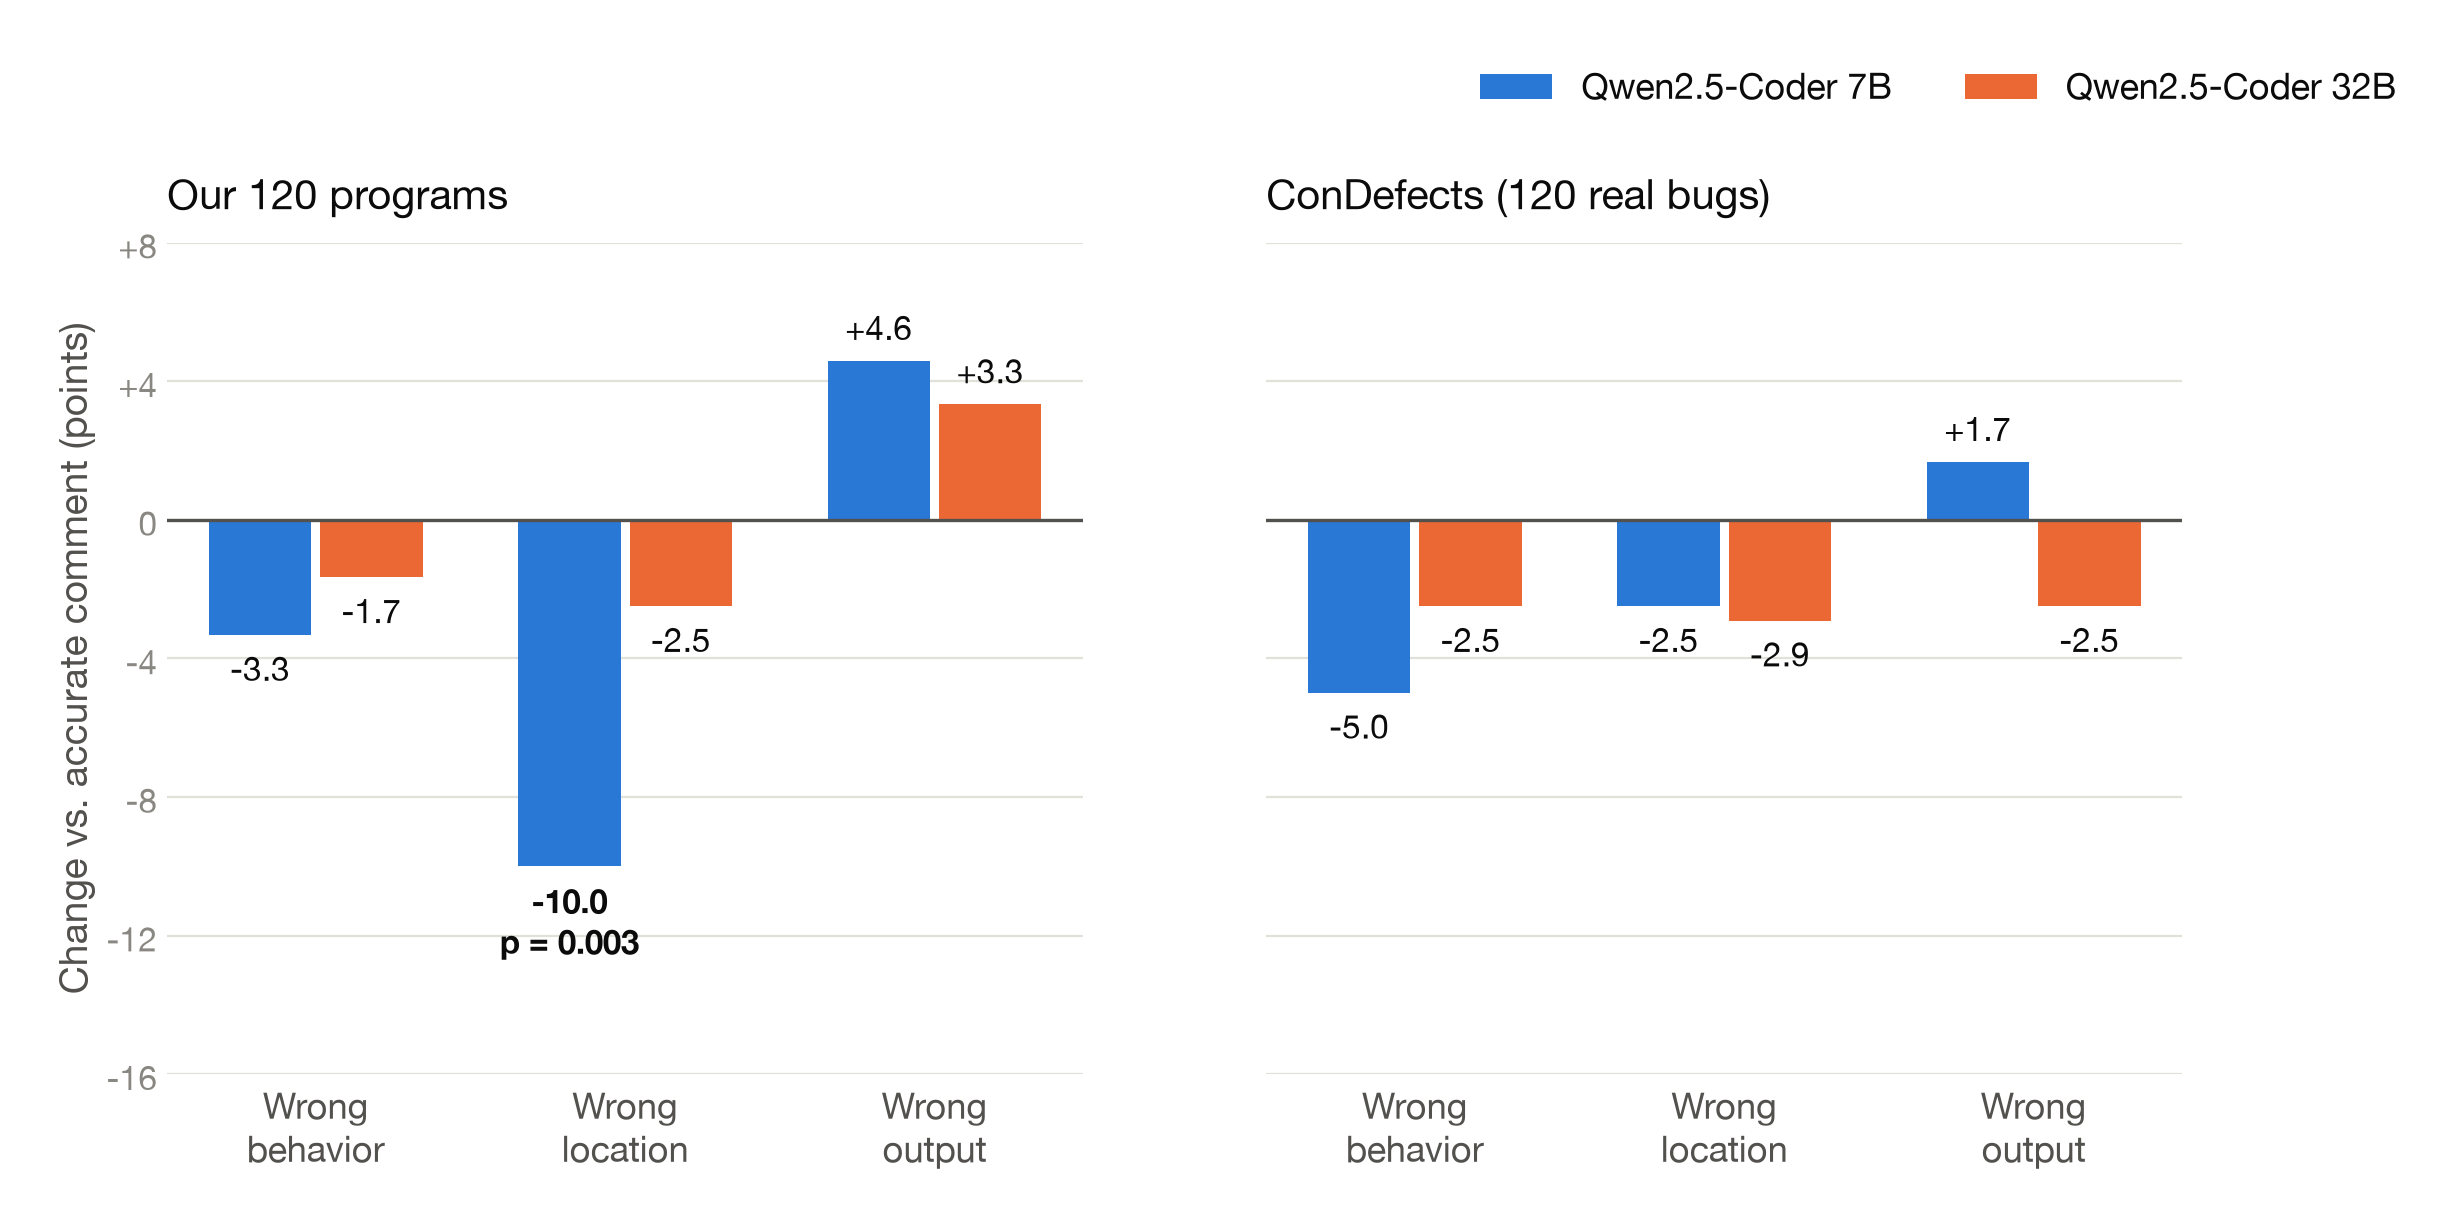
\includegraphics[width=0.85\textwidth]{figures/rq1_change_vs_accurate.png}
\Description{Two bar charts, our programs and ConDefects, showing the change in fix success for each misleading comment relative to the accurate comment for 7B and 32B. The only large bar is 7B with the wrong-location comment on our programs, at minus 10 points with p equal to 0.003; all other bars lie within about 5 points of zero.}
\caption{RQ1: change in fix success compared with the accurate comment, in percentage points (240 pairs per bar). $p$ is shown where $p < 0.05$ (exact McNemar test).}
\label{fig:rq1}
\end{figure*}

\subsection{RQ1: Are Misleading Comments Worse Than Accurate Ones?}
Table~\ref{tab:rq1} gives fix success for each comment version; Table~\ref{tab:mcnemar} and Figure~\ref{fig:rq1} give the paired comparisons.

\paragraph{The larger model fixes more, and real bugs are harder.} With the accurate comment, 32B fixes 85.4\% of our programs and 7B fixes 70.8\%. The real \cd{} bugs are much harder: 71.7\% for 32B and 49.6\% for 7B.

\paragraph{Only the wrong-location comment clearly hurts, and only for 7B.} On our programs, the wrong-location comment lowers 7B's success by 10.0 points (42 programs lost, 18 gained, $p = 0.003$). It is the only result that stays significant after correcting for all 16 comparisons. Across all misleading kinds together, 7B loses 2.9 points ($p = 0.099$) and 32B loses only 0.3 points ($p = 0.904$). On \cd{}, every misleading kind costs 32B 2.5--2.9 points, and 7B changes by between $-5.0$ and $+1.7$ points, but none of these differences is significant. Across all kinds, 7B loses 1.9 points and 32B 2.6 points.

\paragraph{The wrong-output comment slightly helps on our programs.} We did not expect this: the wrong-output comment raises success on our programs by 4.6 points for 7B and 3.3 points for 32B (not significant). Section~\ref{sec:discussion} discusses a possible reason.

\paragraph{By bug type.} For 7B on our programs, the drop is mostly in wrong-comparison bugs: fixed 75\% of the time with the accurate comment and 65\% with misleading comments. Off-by-one (75\% vs.\ 76\%), missed-edge-case (66\% vs.\ 64\%), and other bugs (68\% vs.\ 67\%) barely change. For 32B, no bug type on our programs changes by more than four points.

\begin{quote}
\textbf{Answer to RQ1:} a misleading comment can make repair worse than an accurate one, but the effect is small. The only significant harm is the wrong-location comment on the 7B model ($-10$ points). The 32B model is mostly unaffected, so model size helps.
\end{quote}

\subsection{RQ2: Which Misleading Kind Does the Most Damage?}

\begin{table}[t]
\caption{RQ2: among failed fixes, the share where the bug survived (\emph{followed}: the fix still gives the buggy code's answers on every test the buggy code fails). Number of failed fixes in parentheses. The accurate comment is the baseline.}
\label{tab:rq2}
\footnotesize
\setlength{\tabcolsep}{5pt}
\begin{tabular}{@{}lrrrr@{}}
\toprule
Model & Accurate & Behavior & Location & Output \\
\midrule
\multicolumn{5}{@{}l}{\emph{Our 120 programs}} \\
7B  & 61\% (70) & 67\% (78) & \textbf{76\% (94)} & 66\% (59) \\
32B & 74\% (35) & 72\% (39) & 78\% (41) & 74\% (27) \\
\midrule
\multicolumn{5}{@{}l}{\emph{\cd{} (120 real bugs)}} \\
7B  & 50\% (121) & 47\% (133) & 47\% (127) & 45\% (117) \\
32B & 53\% (68) & 57\% (74) & 45\% (75) & 43\% (74) \\
\bottomrule
\end{tabular}
\end{table}

Table~\ref{tab:rq2} shows how often the original bug survived when a fix failed. The wrong-location comment is both the most damaging kind in RQ1 and the one that most often leaves the bug in place. After it, 76\% of 7B's failed fixes on our programs still give the buggy answers, compared with 61\% after the accurate comment. Its share of \emph{other errors} drops to match (18\% vs.\ 34\%). In other words, the model believes the buggy part was ``verified'', changes another part of the code, and leaves the real bug alone. The wrong-behavior comment shows a smaller shift in the same direction (67\%).

For 32B, and for both models on \cd{}, the misleading kinds stay close to the accurate baseline. On \cd{}, the bug survives in only about half of the failed fixes whatever the comment, because failed fixes of real programs often break something else. 32B rarely fails on our programs (27--41 failures per comment), so its percentages are based on small numbers.

\begin{quote}
\textbf{Answer to RQ2:} the wrong-location comment does the most damage. It mainly misleads the smaller model, which then edits the wrong place and leaves the real bug in place.
\end{quote}

\begin{figure*}[t]
\centering
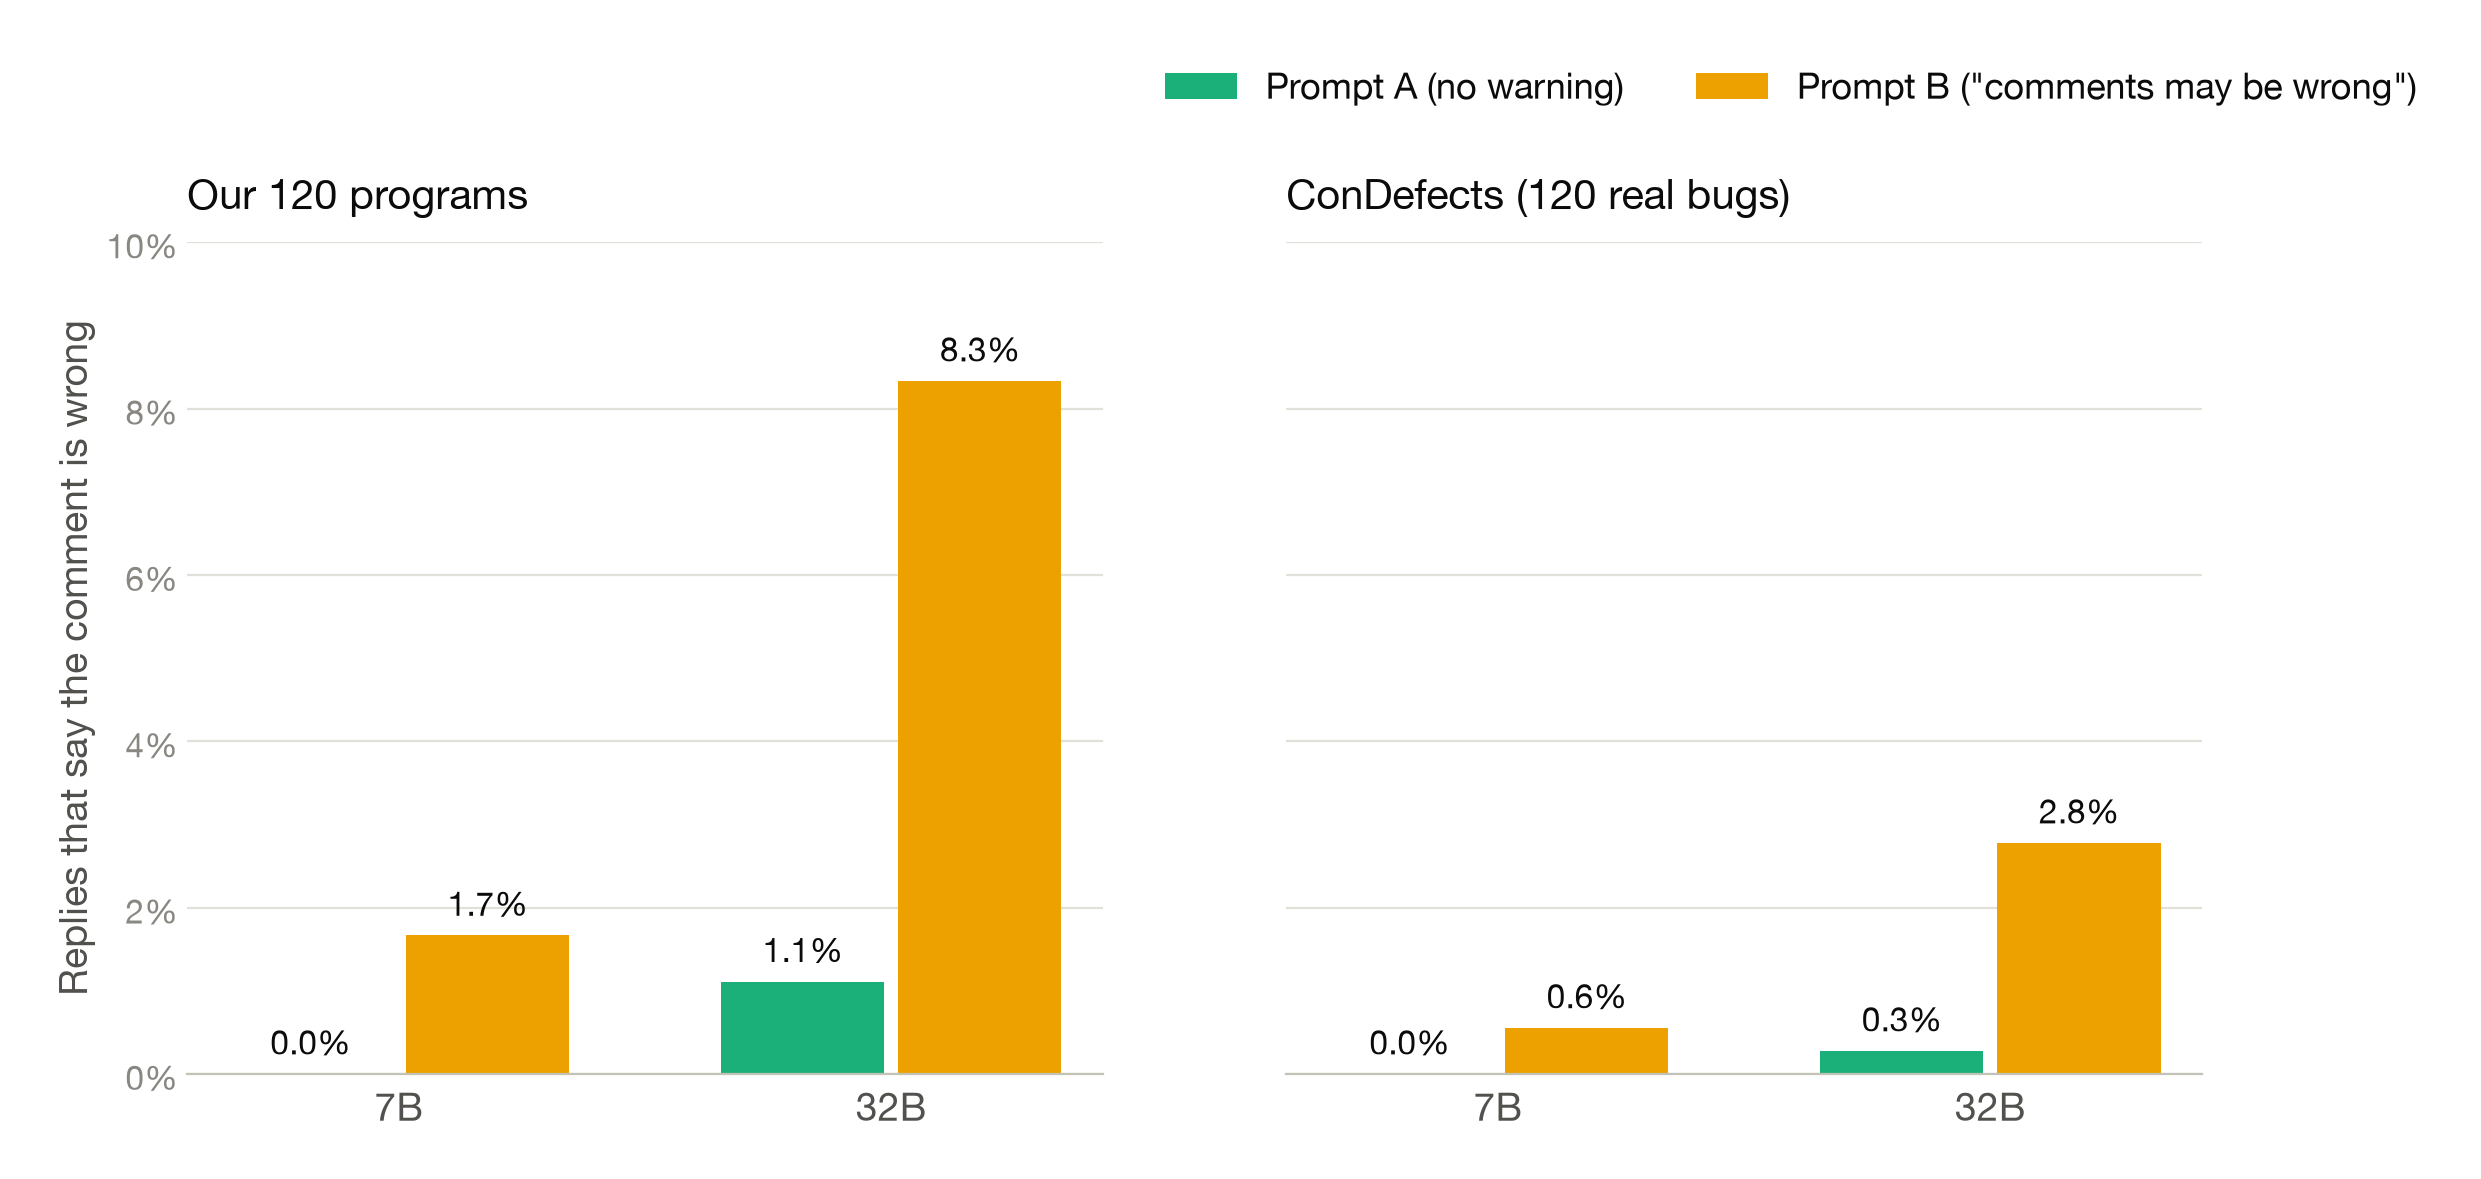
\includegraphics[width=0.85\textwidth]{figures/rq3_flag_rate.png}
\Description{Two bar charts, our programs and ConDefects, showing the share of replies that say the misleading comment is wrong, for 7B and 32B under Prompt A and Prompt B. All bars are below 2 percent except 32B with Prompt B: 8.3 percent on our programs and 2.8 percent on ConDefects.}
\caption{RQ3: share of replies to misleading comments that say the comment is wrong, without (Prompt A) and with (Prompt B) the warning ``the comments in the code may be wrong''; 360 replies per bar.}
\label{fig:rq3}
\end{figure*}

\subsection{RQ3: Do Models Notice the Mismatch, and Does a Warning Help?}

\begin{table}[t]
\caption{RQ3: replies to misleading comments that flag the comment as wrong (of 360 per cell), and fix success with and without the warning (misleading comments only).}
\label{tab:rq3}
\footnotesize
\setlength{\tabcolsep}{5pt}
\begin{tabular}{@{}lrrrr@{}}
\toprule
 & \multicolumn{2}{c}{Flags comment} & \multicolumn{2}{c}{Fix success} \\
\cmidrule(lr){2-3}\cmidrule(lr){4-5}
Model & Prompt A & Prompt B & Prompt A & Prompt B \\
\midrule
\multicolumn{5}{@{}l}{\emph{Our 120 programs}} \\
7B  & 0 (0.0\%) & 6 (1.7\%) & 68.1\% & 67.8\% \\
32B & 4 (1.1\%) & 30 (8.3\%) & 85.3\% & 85.0\% \\
\midrule
\multicolumn{5}{@{}l}{\emph{\cd{} (120 real bugs)}} \\
7B  & 0 (0.0\%) & 2 (0.6\%) & 48.6\% & 46.7\% \\
32B & 1 (0.3\%) & 10 (2.8\%) & 70.0\% & 68.1\% \\
\bottomrule
\end{tabular}
\end{table}

\paragraph{Models almost never question the comment.} Without a warning (Prompt~A), 7B flagged none of the 720 misleading comments across both datasets, and 32B flagged 5 (Table~\ref{tab:rq3}, Figure~\ref{fig:rq3}). Even 32B, which is rarely misled, almost never says the comment is wrong; it just fixes the code.

\paragraph{The warning changes what models say, not what they do.} With the warning (Prompt~B), 32B flags 8.3\% of misleading comments on our programs and 2.8\% on \cd{}; 7B flags at most 1.7\%. But fix success does not change. On our programs, 7B fixes 245 vs.\ 244 of 360 misleading-comment cases with Prompts A and B, and 32B fixes 307 vs.\ 306 ($p = 1.000$ for both, and also $p = 1.000$ for the accurate comment). On \cd{}, success with misleading comments is slightly lower with the warning (7B $-1.9$, 32B $-1.9$ points; $p = 0.44$ and $0.32$). The only effect of the warning with $p < 0.05$ is an \emph{improvement} for 32B with the accurate comment on \cd{} (69\% $\to$ 74\%: 6 fixes gained, none lost; $p = 0.031$), which does not pass the correction for multiple tests.

\paragraph{Flagging is not fixing.} On our programs, 19 of the 40 replies that flagged the comment still failed the tests; 7B fixed only 2 of the 6 bugs where it called out the comment. In several of these replies the model ``fixed'' the comment and left the code as it was.

\begin{quote}
\textbf{Answer to RQ3:} models rarely notice that a comment does not match the code. Warning them that comments may be wrong makes the larger model mention it more often, but does not make either model fix more bugs.
\end{quote}

\subsection{Memorization Check}

\begin{table}[t]
\caption{Memorization check: given the code before the buggy line, how closely does the model continue the real program? Median similarity (0--1) and number of programs (of 120) where it writes the exact fixed or buggy line.}
\label{tab:memo}
\footnotesize
\setlength{\tabcolsep}{5pt}
\begin{tabular}{@{}llrrr@{}}
\toprule
Model & Dataset & Similarity & Fixed line & Buggy line \\
\midrule
7B  & \cd{} (public)     & 0.44 & 15 & 11 \\
    & Ours (never seen)  & 0.59 & 22 & 6 \\
\midrule
32B & \cd{} (public)     & 0.44 & 20 & 10 \\
    & Ours (never seen)  & 0.52 & 22 & 12 \\
\bottomrule
\end{tabular}
\end{table}

If the models had memorized the \cd{} programs, they would continue them more closely than our never-seen programs. Table~\ref{tab:memo} shows the opposite. Median similarity is lower for \cd{} (0.44 vs.\ 0.59 for 7B, 0.44 vs.\ 0.52 for 32B), and the exact fixed line does not appear more often. The exact buggy line appears somewhat more often for 7B (11 vs.\ 6 programs) but not for 32B (10 vs.\ 12), and these counts are small. We find no sign of memorization. Our programs are probably easier to continue because they are written in a clean, predictable style with descriptive names, while contest code is short and quirky.

\subsection{Case Studies}
\label{sec:cases}
Three replies on our programs show what these numbers look like in practice. We chose the clearest example of each pattern; each one behaves the same under both prompts unless noted.

\paragraph{The wrong-location comment moves the fix.} \texttt{sprouts\_per\_column} receives a seed tray as a list of rows of booleans and should count the sprouted seeds in each column. Its loop runs over \texttt{range(len(tray))}, the number of rows, instead of the number of columns. With the accurate comment, 7B finds this under both prompts and loops over \texttt{len(tray[0])}. With the wrong-location comment
\casecomment{Column loop checked; the sprout test may miss cells stored as 1 instead of True}
it keeps the loop and changes the sprout test to \texttt{row[c] is True}, saying that cells stored as \texttt{1} should not count. The loop bug survives: on every test the buggy code fails, the ``fixed'' code gives the same wrong answers. The comment did more than distract the model: it suggested a believable bug, and the model fixed that one instead.

\paragraph{Flagging is not fixing.} In \texttt{chapter\_lengths}, each chapter is taken to end on the first page of the next chapter instead of the page before it, so every chapter but the last is one page too long. The wrong-location comment reads
\casecomment{Chapter ends verified; check the length formula end - start + 1}
Under Prompt~B, 32B replies that ``the bug is in the comment'', which suggests ``that the ends are verified, which they are not''. It then says ``the code itself is correct'' and returns the code unchanged with a rewritten comment. The judge rightly counts this as flagging the comment, and the model's doubt even points at the real problem, but the bug stays. (32B fails this program with every comment, including the accurate one, so the comment did not cause the failure here; the example only shows that noticing a false comment does not lead to a fix.)

\paragraph{A false example acts as a failing test.} \texttt{archive\_decades} should count the calendar decades from the earliest to the latest recording, but computes \texttt{(last - first) // 10 + 1}, which counts ten-year spans: 1975 to 1984 gives 1 instead of 2. With the accurate comment, 7B fails under both prompts, returning the formula unchanged (Prompt~A) or adding a special case (Prompt~B). With the wrong-output comment
\casecomment{Example: archive\_decades([1975, 1984]) returns 1}
it rewrites the formula as \texttt{last // 10 - first // 10 + 1} and passes every test under both prompts, even though its fix returns 2 for that same input and so disagrees with the example. The example's answer is wrong, but its input is exactly a case where the code goes wrong, and the model seems to use that input.

% ---------------------------------------------------------------------------
\section{Discussion}
\label{sec:discussion}

\paragraph{Where a comment points matters more than whether it is true.} The two comments that point somewhere behave in opposite ways. The wrong-location comment points \emph{away} from the bug and is the only kind that clearly hurts. The wrong-output comment is also false (its ``expected'' value is the buggy output), yet it slightly helps, possibly because its example names an input on which the code goes wrong, so it works like a failing test (Section~\ref{sec:cases}). The wrong-behavior comment, which describes the bug as intended but does not point anywhere, falls between the two. So for these models, comments seem to matter mostly as a guide to \emph{where to look}.

\paragraph{Robust, but not aware.} The 32B model is barely affected by any misleading comment, yet almost never says that a comment is wrong. Its robustness seems to come from understanding the code and problem description well enough that the comment rarely matters, not from checking the comment against the code. A model that trusts comments this much is still at risk when the code alone is not enough, which is exactly when a well-placed misleading comment, or an out-of-date one, would do the most harm.

\paragraph{Why the warning does not help.} A general warning tells the model that \emph{some} comment may be wrong, but not which part of the code to distrust. The model mentions the possibility more often, but its fix stays the same. This suggests that repair tools should check comments against the code directly instead of relying on a warning in the prompt.

\paragraph{Planted versus real bugs.} On \cd{} the effects are smaller and not significant, although every misleading kind still costs 32B a few points. Real bugs are harder to begin with, and in a whole contest program a single comment at the top has less influence than a comment inside a short function. Whether the effect of comments grows or shrinks with program size is an open question.

\paragraph{Implications.} For developers, the risk from a misleading comment in AI-assisted bug fixing is small with a strong model, but not zero: fixes in code whose comments may be out of date deserve a second look, especially with a smaller model. For tool builders, models do not reliably notice when a comment contradicts the code, so checking comments is worth doing as a separate step. For security, changing a single comment was enough to steer the smaller model away from the bug in a measurable share of cases.

\paragraph{Lessons learned.} A pilot run was essential: our first programs were too easy to show any effect, which led us to subtler bugs and a fourth bug type. Free cloud GPUs were enough for all 3,840 repairs, but each notebook installed the latest Ollama, so versions differed between team members; next time we would fix the version. An LLM judge plus a targeted hand check labeled 2,880 replies for a few dollars. Real bugs needed whole-program input/output testing, a time limit, and a memorization check.

% ---------------------------------------------------------------------------
\section{Threats to Validity}
\label{sec:threats}

\paragraph{Construct validity (do we measure the right thing?).} Success is defined by tests, and weak tests could accept a wrong fix. Each of our programs has at least five tests; the correct code passes all of them and the buggy code fails at least one. \cd{} uses AtCoder's official tests. RQ2's \emph{followed} label shows whether the buggy behavior survived, not why. RQ3 measures what models \emph{say}; a model may notice a mismatch without mentioning it. The RQ3 judge was checked by hand on 620 labels and all were confirmed, but the checkers could see the judge's labels, so this shows confirmation, not independent agreement.

\paragraph{Internal validity (could something else explain the results?).} An LLM wrote the comments following fixed rules, and we did not rate each one for how convincing it is; some misleading comments may be more convincing than others. Our 108 generated programs come from one model (Claude Opus 5.5) and may share its habits, and eight pairs of programs use similar bug tricks. We use temperature 0 and one run per version instead of several random runs. The 7B model gave identical replies when rerun, while the 32B model, split across two GPUs, sometimes reworded a reply but with the same result. Ollama versions ranged from 0.40.13 to 0.40.16 across runs. One correct but slow \cd{} fix (\texttt{abc264\_c}, 32B) went over the 10-second limit on Kaggle and is counted as a failure.

\paragraph{External validity (do the results generalize?).} We test one open model family (Qwen2.5-Coder), in 4-bit quantized form, and only Python. Our programs are short functions with a one-line comment; longer comments, docstrings, several conflicting comments, or AI agents that can run tests may behave differently. We used 120 programs per dataset, fewer than the 150--200 first planned, and we dropped the no-comment version, so we cannot say how much an accurate comment helps compared with no comment.

\paragraph{Conclusion validity (are the statistics strong enough?).} With 240 pairs per comparison, our tests can detect differences of several percentage points but may miss smaller ones, such as the steady 2--3-point losses on \cd{}. We report raw $p$-values for the 16 RQ1 comparisons and mark the one that passes the Bonferroni correction.

% ---------------------------------------------------------------------------
\section{Conclusion}
We asked whether a misleading comment can trick an LLM into a wrong bug fix. Across 3,840 repair attempts on new and real bugs, a misleading comment is a small risk overall. It mainly hurts the smaller model, and most when it points away from the bug; the model then tends to leave the real bug alone. The larger model is barely affected. At the same time, models almost never say that a comment is wrong, and warning them that comments may be wrong does not help them fix more bugs. Future work should test other model families, including closed models, longer comments and docstrings, AI agents that can run tests, and repair tools that check comments against the code.

\section*{Data Availability}
All programs, tests, comments, prompts, model replies, labels, analysis scripts, and notebooks are available in our repository: \url{https://github.com/ankit-bhade/misleading-comments}. The README explains how to reproduce every table and figure in this report.

\bibliographystyle{ACM-Reference-Format}
\bibliography{references}

\end{document}
